% !TeX spellcheck = en_GB
% encoding: utf8
% !TEX encoding = utf8
% !TEX program = pdflatex
% !BIB program = biber

\documentclass[11pt,oneside,a4paper]{report}

\usepackage[utf8]{inputenc}
\usepackage[T1]{fontenc}
\usepackage[colorlinks]{hyperref}
\usepackage[left=2.5cm, right=2.5cm, top=2.5cm, bottom=2.5cm]{geometry}
\usepackage{float}
\usepackage{subcaption}
\usepackage{mathtools}
\usepackage{color}
\usepackage{listings}
\usepackage{xcolor}
\usepackage[backend=biber,maxnames=10,style=numeric,sorting=nty,abbreviate=false,giveninits=true,language=english]{biblatex}

\addbibresource{../meros.bib}

%\newcommand{\twc}[1]{\textcolor{red}{\textbf{TW}: #1}}
\newcommand{\Fig}[1]{Fig.~\ref{#1}}

\definecolor{amber}{rgb}{1.0, 0.49, 0.0}
\newcommand{\twci}[1]{
	\textcolor{amber}{TW: #1}}

% encoding: utf8
%
% Stereotypes
%

% Lista powinna być zgodna z profilem w EA

\newcommand{\stActionConn}{<<Action>>}
\newcommand{\stCommChannel}{<<CommChannel>>}
\newcommand{\stComponContain}{<<ComponContain>>}
\newcommand{\stGpPackages}{<<GpPackages>>}
\newcommand{\stHardware}{<<Hardware>>}
\newcommand{\stLaunchFile}{<<LaunchFile>>}
\newcommand{\stMetaPackage}{<<MetaPackage>>}
\newcommand{\stMicroNode}{<<MicroNode>>}
\newcommand{\stNamespace}{<<Namespace>>}
\newcommand{\stNode}{<<Node>>}
\newcommand{\stPackage}{<<Package>>}
\newcommand{\stParameter}{<<Parameter>>}
\newcommand{\stRepository}{<<Repository>>}
\newcommand{\stRosCommCompon}{<<RosCommCompon>>}
\newcommand{\stRosConn}{<<RosConn>>}
\newcommand{\stRQtNode}{<<RQtNode>>}
\newcommand{\stRunSystemCompon}{<<RunSystemCompon>>}
\newcommand{\stServiceConn}{<<Service>>}
\newcommand{\stSourExeContain}{<<SourExeContain>>}
\newcommand{\stSystem}{<<System>>}
\newcommand{\stTerminal}{<<Terminal>>}
\newcommand{\stTopicConn}{<<Topic>>}
\newcommand{\stWorkspace}{<<Workspace>>}

\newcommand{\stblock}{<<block>>}






\lstdefinestyle{terminal}{
	backgroundcolor=\color{darkgray},
	basicstyle=\ttfamily\color{green}\footnotesize,
	frame=single,
	rulecolor=\color{gray},
}


\begin{document}
	
\title{MeROS: basics of metamodel usage with turtlesim}
\author{MeROS developers group - https://github.com/twiniars/MeROS \\ tomasz.winiarski@pw.edu.pl}
\date{\today}
\maketitle

	
	
	\maketitle
	

	
\chapter*{Important citation notice}

\textbf{If you are to use MeROS in your papers, please first cite the IEEE ACCESS  article~\cite{meros-access}, where the initial version of the MeROS is presented. You can also refer to MeROS project page \cite{meros-www} and mention the actual MeROS version you are using.}
	
\chapter{Introduction}
\label{ch:introduction}

	This document is to present some basics of MeROS metamodel usage (its application). It bases on popular turtlesim ROS2 tutorial \url{https://docs.ros.org/en/jazzy/Tutorials/Beginner-CLI-Tools.html} and has an introspection, reverse engineering nature. The procedure of the new systems creation with V-model and MerROS is presented in \cite{winiarski2025-v-model}.

\chapter{MeROS application}
\label{ch:application}


The MeROS \stSystem{} structure presentation is composed by different views on it. In this example we start with Sources and Executables composition into the System. It should be noted that tourtlesim package should be installed before as well as  source command should be executed properly in each system console.

\begin{lstlisting}[style=terminal]
$ ros2 pkg executables turtlesim
turtlesim draw_square
turtlesim mimic
turtlesim turtle_teleop_key
turtlesim turtlesim_node
\end{lstlisting}

There are four executables in the turtlesim \stPackage{} that can be treated as \stNode{}s. They are composed into the ROS 2 \stWorkspace{} localised in /opt directory (Fig.~\ref{fig:system_sourexec_composition_bdd}).


\begin{figure}[H]
	\centering
	\begin{center}
		{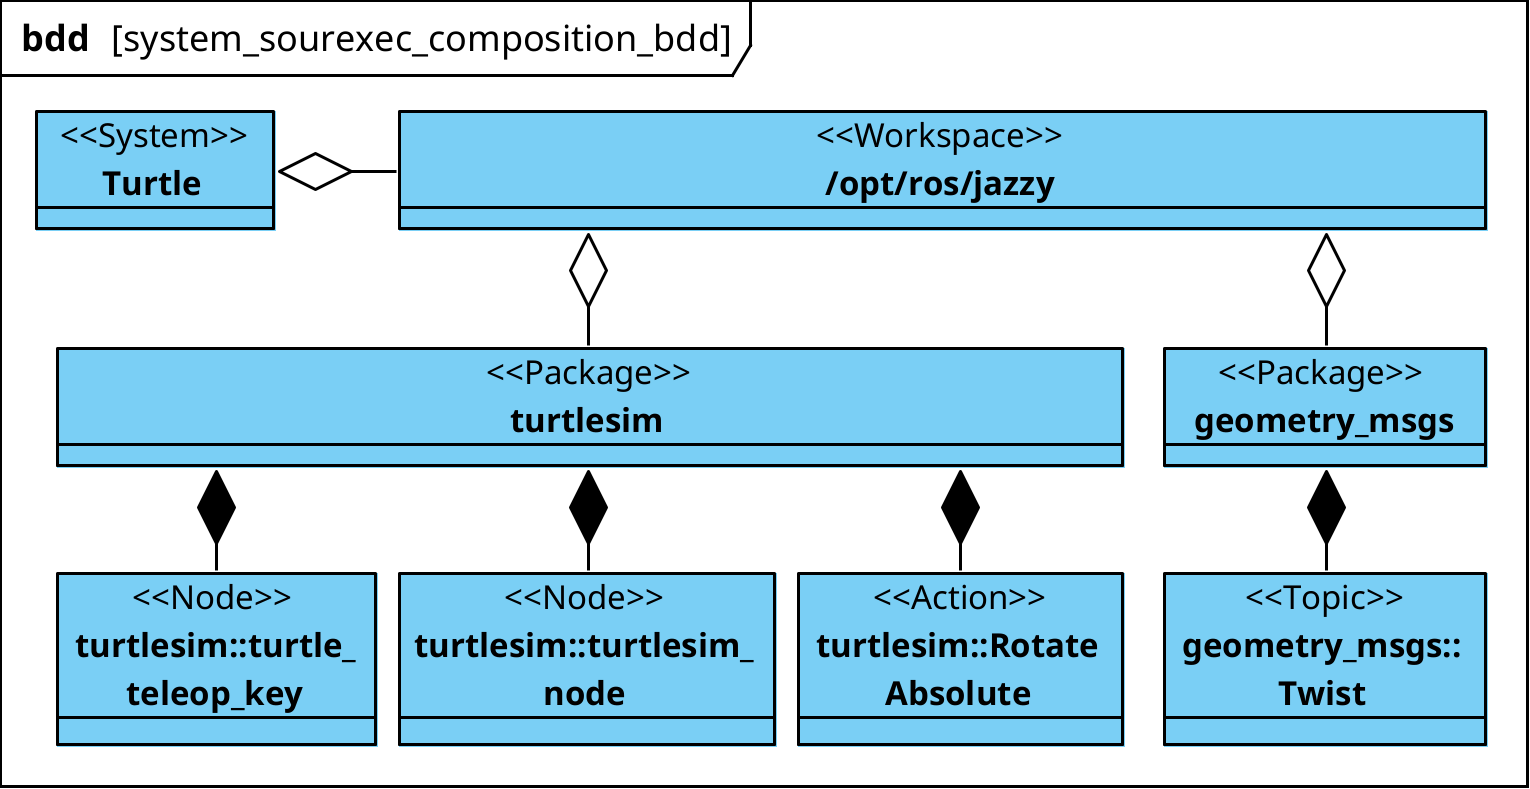
\includegraphics[scale=1.0]{diagrams/system_sourexec_composition_bdd.png}}
	\end{center}
	\caption{System sources and executables composition}
	\label{fig:system_sourexec_composition_bdd}
\end{figure}

	
\chapter{Old MeROS application - to be removed}
\label{ch:application}
	

	

	
	This documentation presents key aspects of an exemplary system development process incorporating MeROS. The exemplary system was created within the AAL INCARE project to control the Rico assistive robot (modified TIAGo platform with controller based on ROS~1) to execute transportation attendance tasks (Fig.~\ref{fig:herbatka_u_winiara}).
	
	\begin{figure}[H]
		\centering
		\begin{center}
			{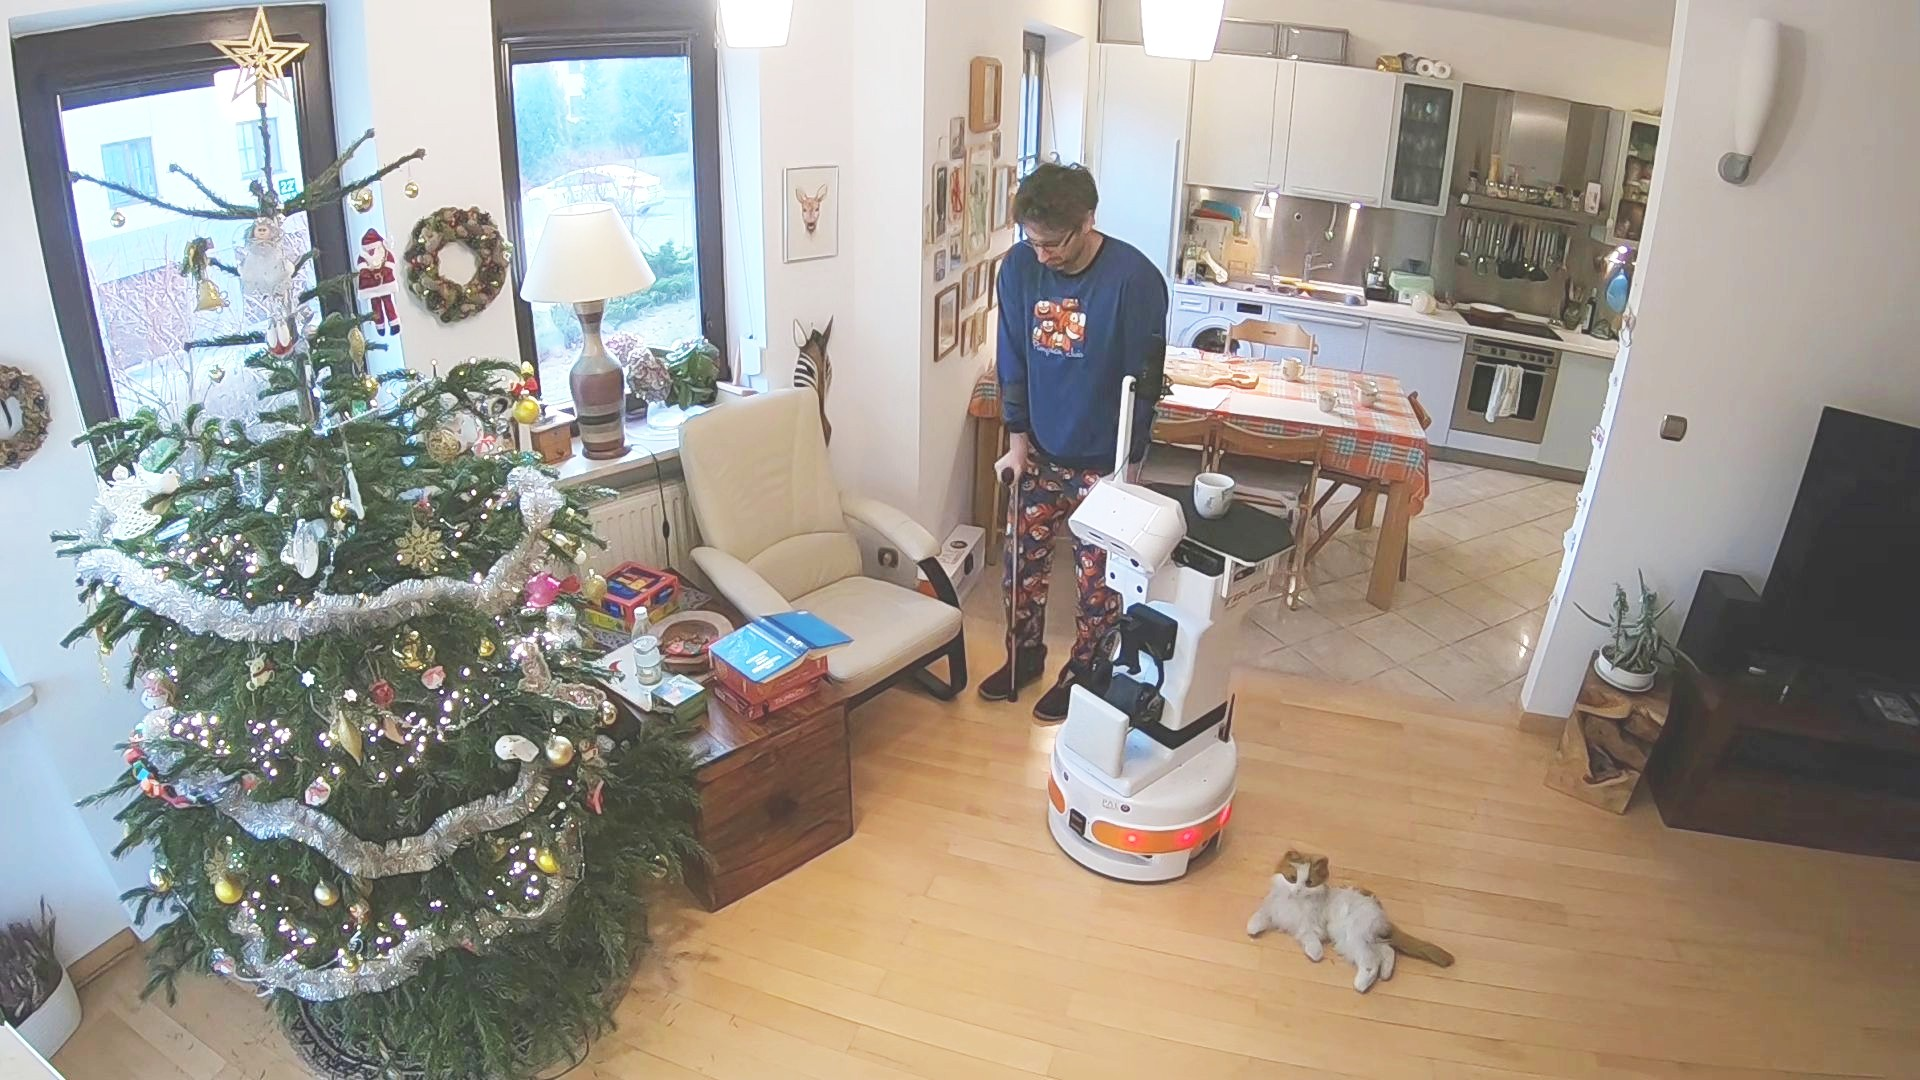
\includegraphics[width=\columnwidth]{img/herbatka_u_winiara.jpg}}
		\end{center}
		\caption{Transportation attendance by Rico robot \url{https://vimeo.com/670252925}} 
		\label{fig:herbatka_u_winiara}
	\end{figure}
	
	
	
	 The purpose of the following description is not to document the entire system but to illustrate, by example, representative aspects of the MeROS application.
	 
	\newpage
	The Rico \stSystem{} consists of two parts. Its \stWorkspace{} and a~number of \stRunSystemCompon{} (Fig.~\ref{fig:rico_system_bdd}).
	
	
	\begin{figure}[H] 
		\centering
		\begin{center}
			{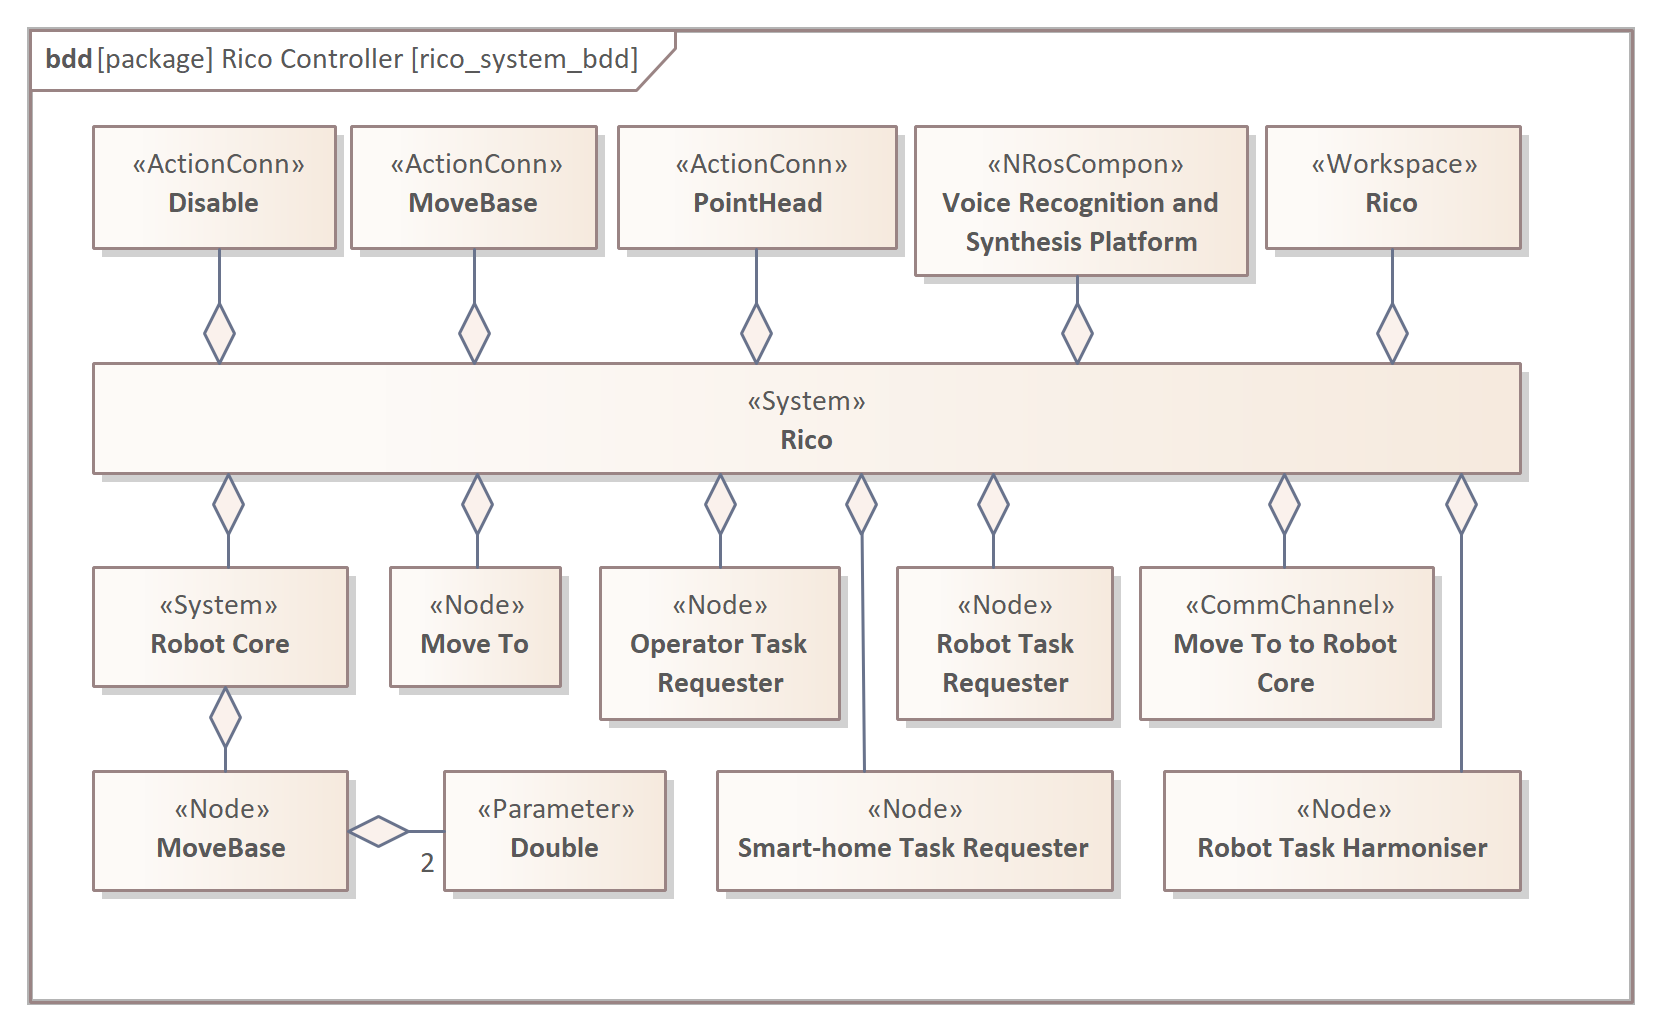
\includegraphics[scale=.9]{img/rico_pkg/rico_system_bdd.png}}
		\end{center}
		\caption{Rico \stSystem{} composition.} 
		\label{fig:rico_system_bdd}
	\end{figure}
	
	
	The fragment of the application scenario is conceptually presented in Fig.~\ref{fig:general_sd}.
	

	\begin{figure}[H] 
		\centering
		\begin{center}
			{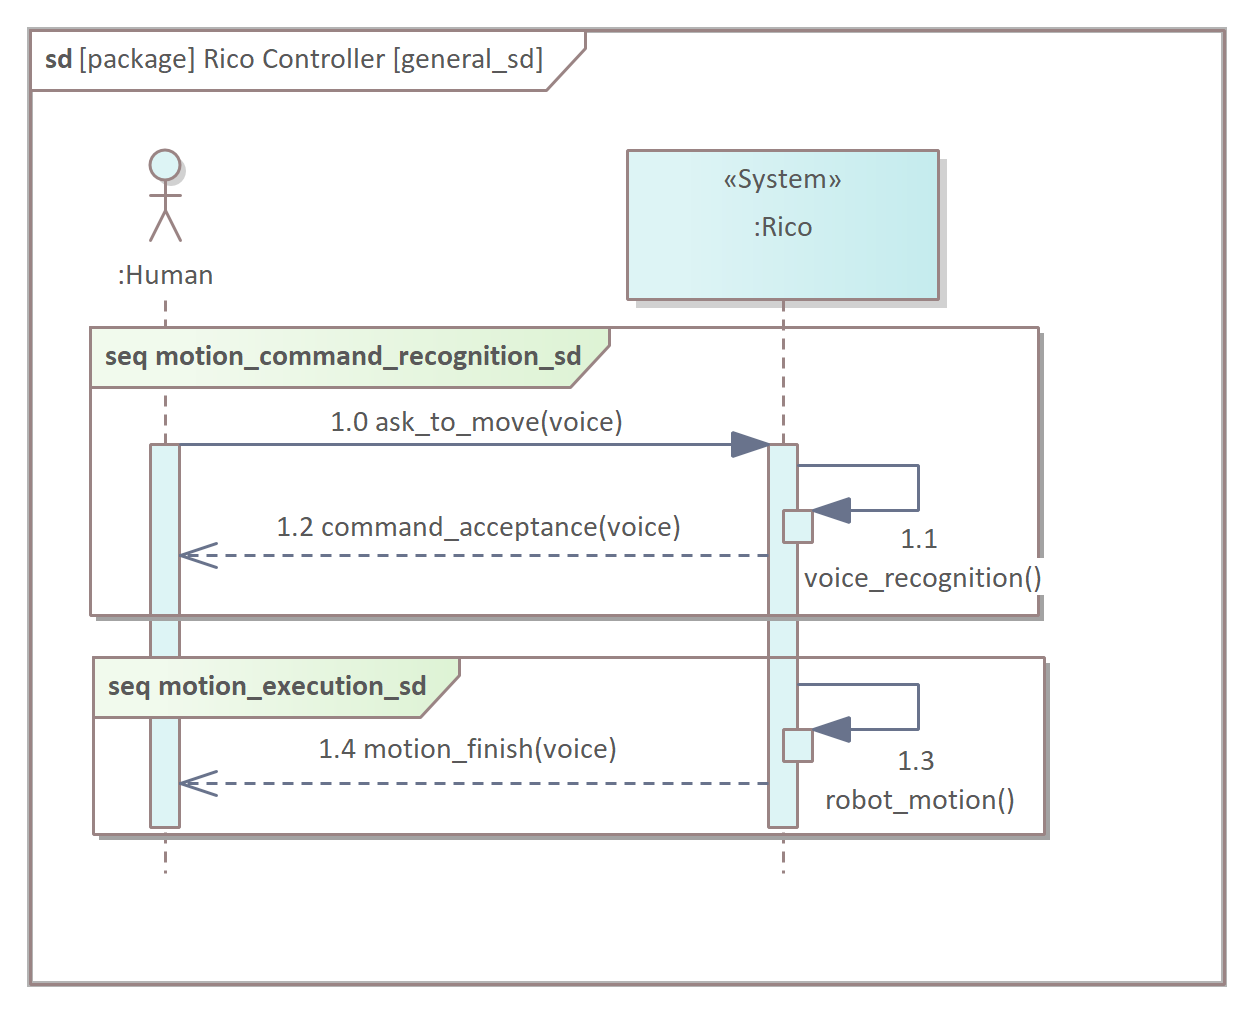
\includegraphics[scale=.9]{img/rico_pkg/general_sd.png}}
		\end{center}
		\caption{Concept scenario.} 
		\label{fig:general_sd}
	\end{figure}
	
	Here, the system (\stSystem{} \texttt{:Rico}) and its behaviour are formulated in a~general way. An actor (e.g. an elderly person) asks the robot to move. Then, the system recognises the voice command and vocally confirms the command's acceptance. Finally, the robot executes the motion and vocally informs that the motion is finished.
	In the following part of the description, the \stSystem{} \texttt{:Rico} and sequence diagram frame \texttt{motion execution} from Fig.~\ref{fig:general_sd} are presented in a~explicit way.
	
		The \stSystem{} \texttt{:Rico} structure is depicted in Fig.~\ref{fig:rico_system_ibd}. Here, and in the following diagrams, the \texttt{rosout} and \texttt{ROS master} \stNode{}s were omitted to make the diagrams more compact. Dedicated block is needed for \stCommChannel{} \texttt{:Move To to Robot Core}, because this \stCommChannel{} is specified in detail later on.
	
	\begin{figure}[H]
		\centering
		\begin{center}
			{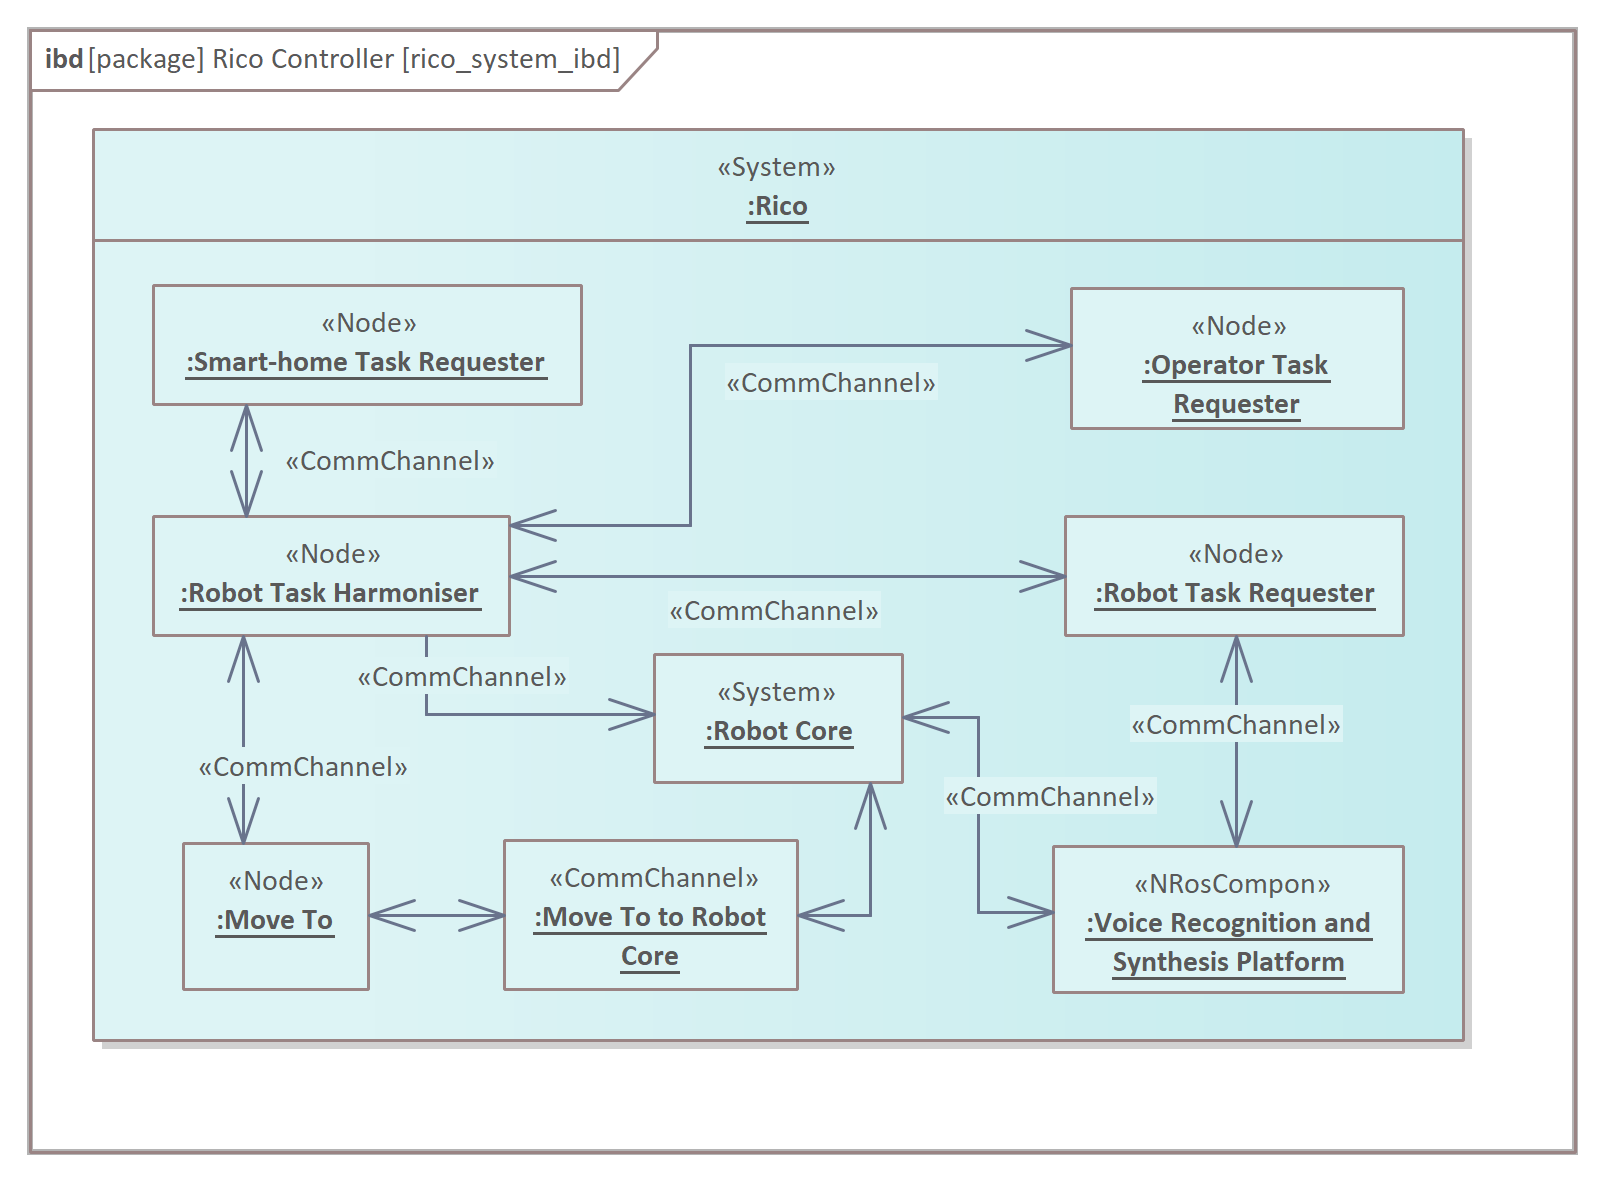
\includegraphics[scale=0.85]{img/rico_pkg/rico_system_ibd.png}}
		\end{center}
		\caption{Structure of \stSystem{}\texttt{:Rico}.} 
		\label{fig:rico_system_ibd}
	\end{figure}

	The system is based on TaskER framework \cite{tasker2020} developed from the RAPP approach to construct systems with variable structure \cite{zielinski2017variable}. The role of the TaskER is to schedule a~robot’s tasks. It consists of (i) Task Requesters \stNode{}s to submit new tasks, (ii) Task Harmoniser \stNode{} to schedule tasks execution, (iii) dynamic \stNode{}s (here, \stNode{} \texttt{:Move To}) to execute a~particular task on the robot hardware and (iv) cloud part, here <<NRosCompon>> \texttt{:Voice Recognition and Synthesis Platform}. The common part of the controller is located in \stSystem{} \texttt{:Rico}.
	
	Fig.~\ref{fig:robot_core_ibd} illustrates how various instances of the same block are depicted in the model. Two \stParameter{} Objects of the same classifier \texttt{:Double} are composed into \stNode{} \texttt{:MoveBase}.
	
	\begin{figure}[H]
		\centering
		\begin{center}
			{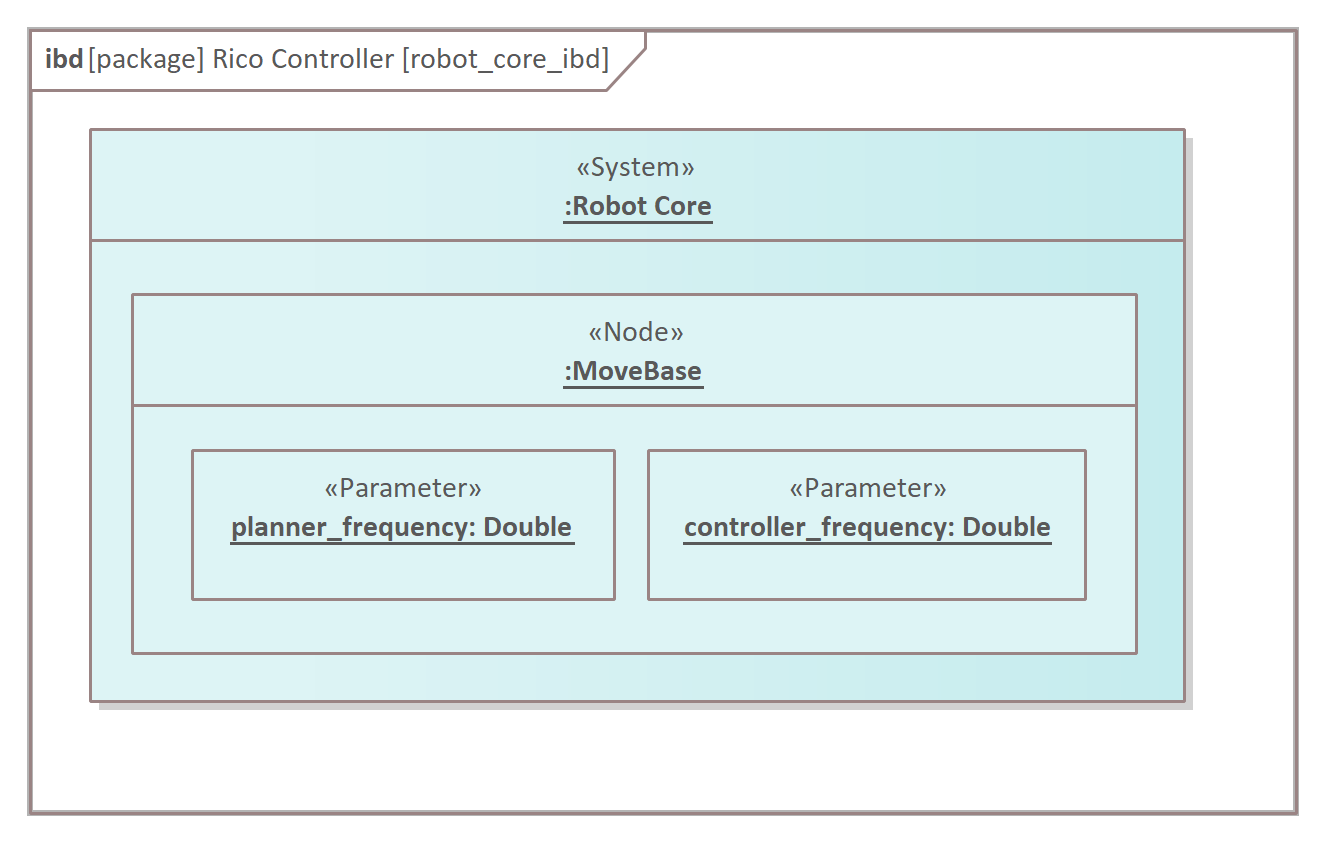
\includegraphics[scale=.85]{img/rico_pkg/robot_core_ibd.png}}
		\end{center}
		\caption{Selected elements of \stSystem{} \texttt{:Robot Core}.} 
		\label{fig:robot_core_ibd}
	\end{figure}
				
	\stCommChannel{} \texttt{:Move To to Robot Core} is depicted in Fig.~\ref{fig:move_to_2_core_cm_ibd}. It comprises three actions.
	

	\begin{figure}[H]
		\centering
		\begin{center}
			{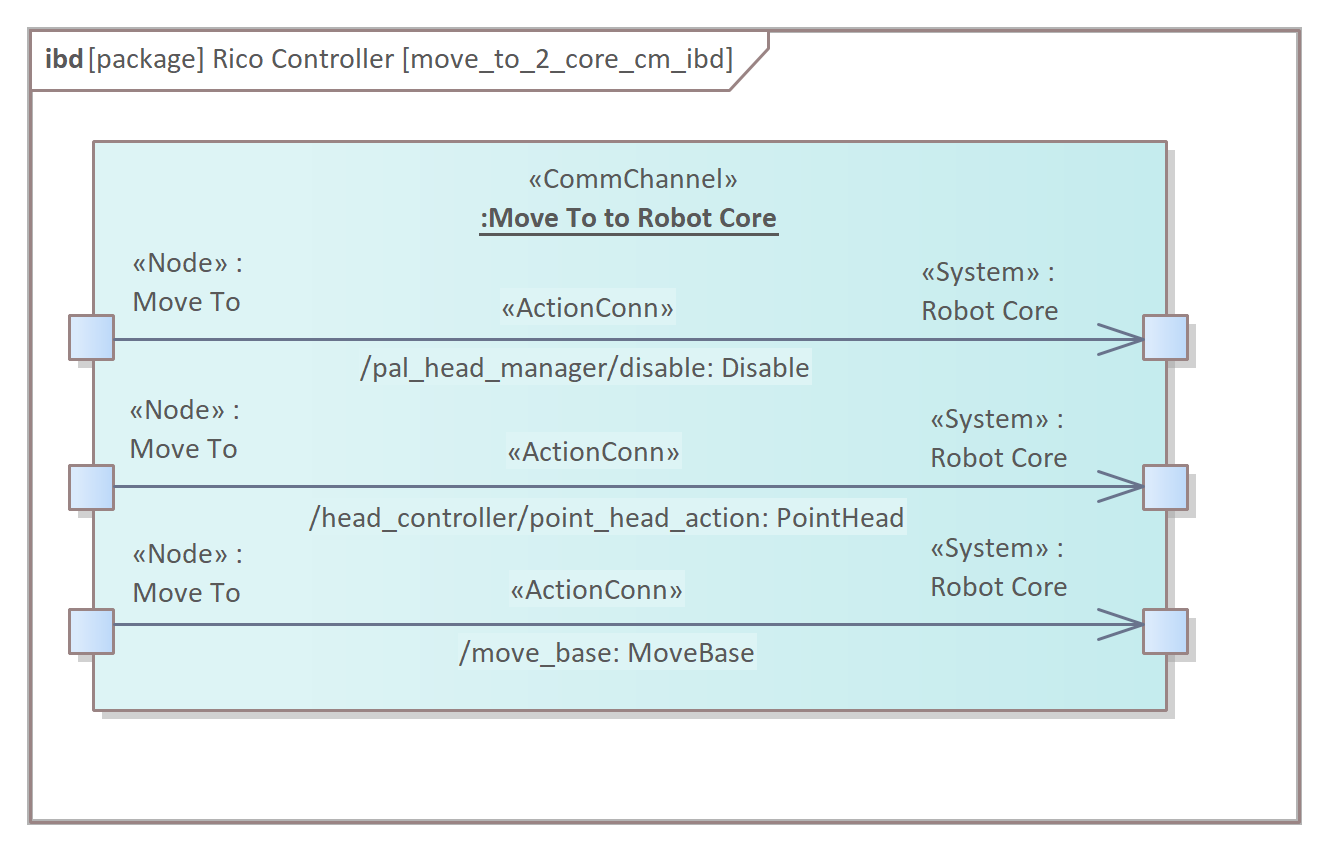
\includegraphics[scale=1.1]{img/rico_pkg/move_to_2_core_cm_ibd.png}}
		\end{center}
		\caption{Example of \stCommChannel{}.} 
		\label{fig:move_to_2_core_cm_ibd}
	\end{figure}
	
		
	The part of the scenario generally described in Fig.~\ref{fig:general_sd} is depicted in detail in Fig.~\ref{fig:motion_execution_sd}. The presentation remains conceptual from the behavioural point of view, but it considers the particular parts of the \stSystem{} \texttt{:Rico}.
	
	\begin{figure}[H]
		\centering
		\begin{center}
			{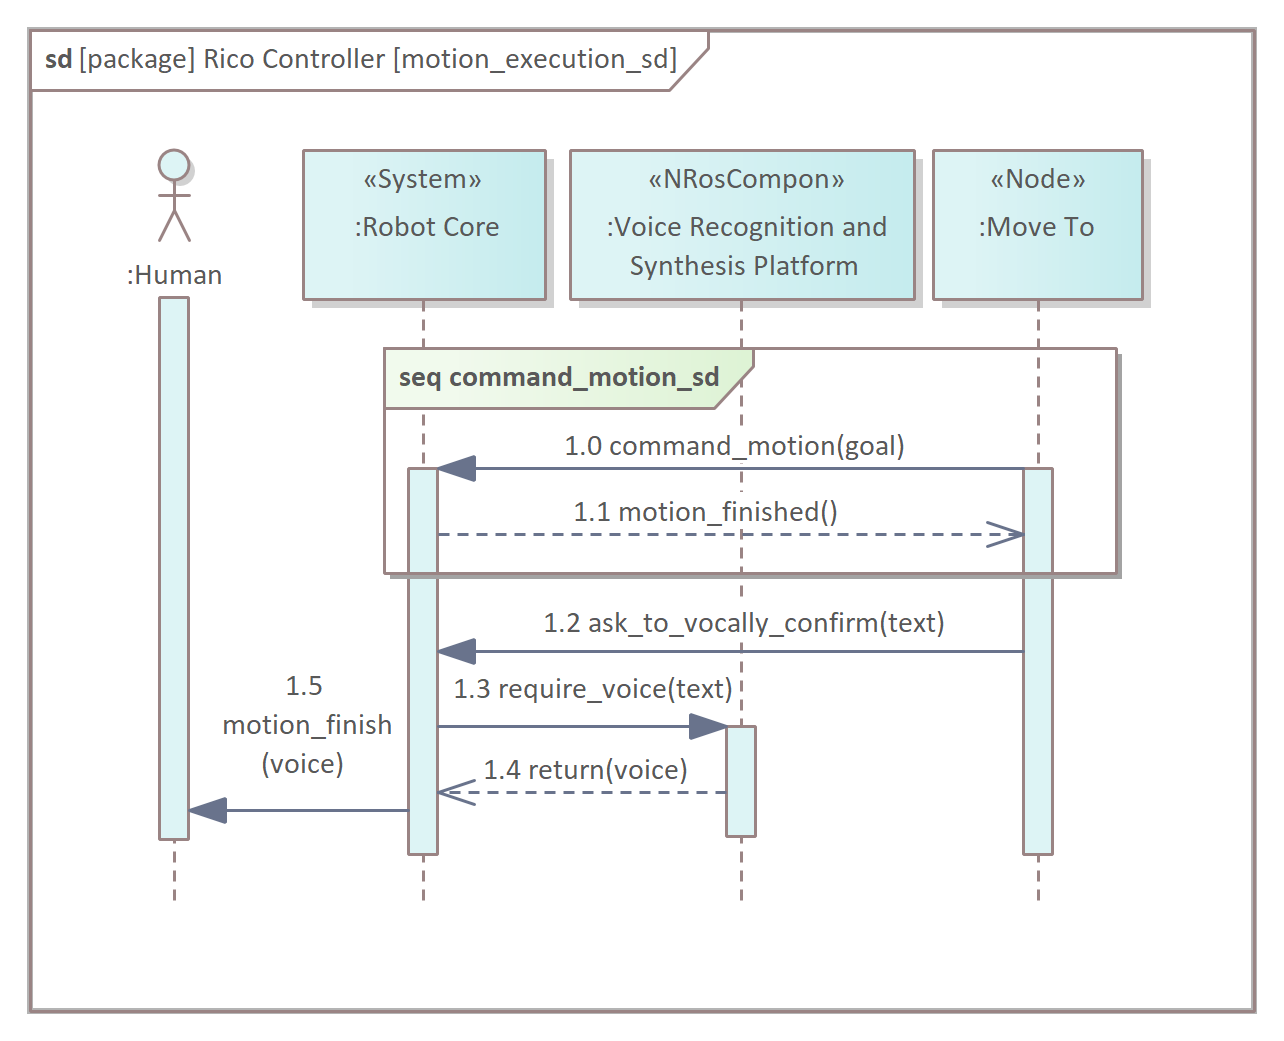
\includegraphics[scale=1.1]{img/rico_pkg/motion_execution_sd.png}}
		\end{center}
		\caption{Motion execution operation.} 
		\label{fig:motion_execution_sd}
	\end{figure}


	Finally, the particular communication methods are specified on the most detailed, ROS-specific level (Fig.~\ref{fig:command_motion_sd}). The command\_motion operation includes the sequence of four steps of communication. Three Actions realise the communication, one utilised twice. The diagram comprises extra notes that make it easier to interpret.
	
	\begin{figure}[H]
		\centering
		\begin{center}
			{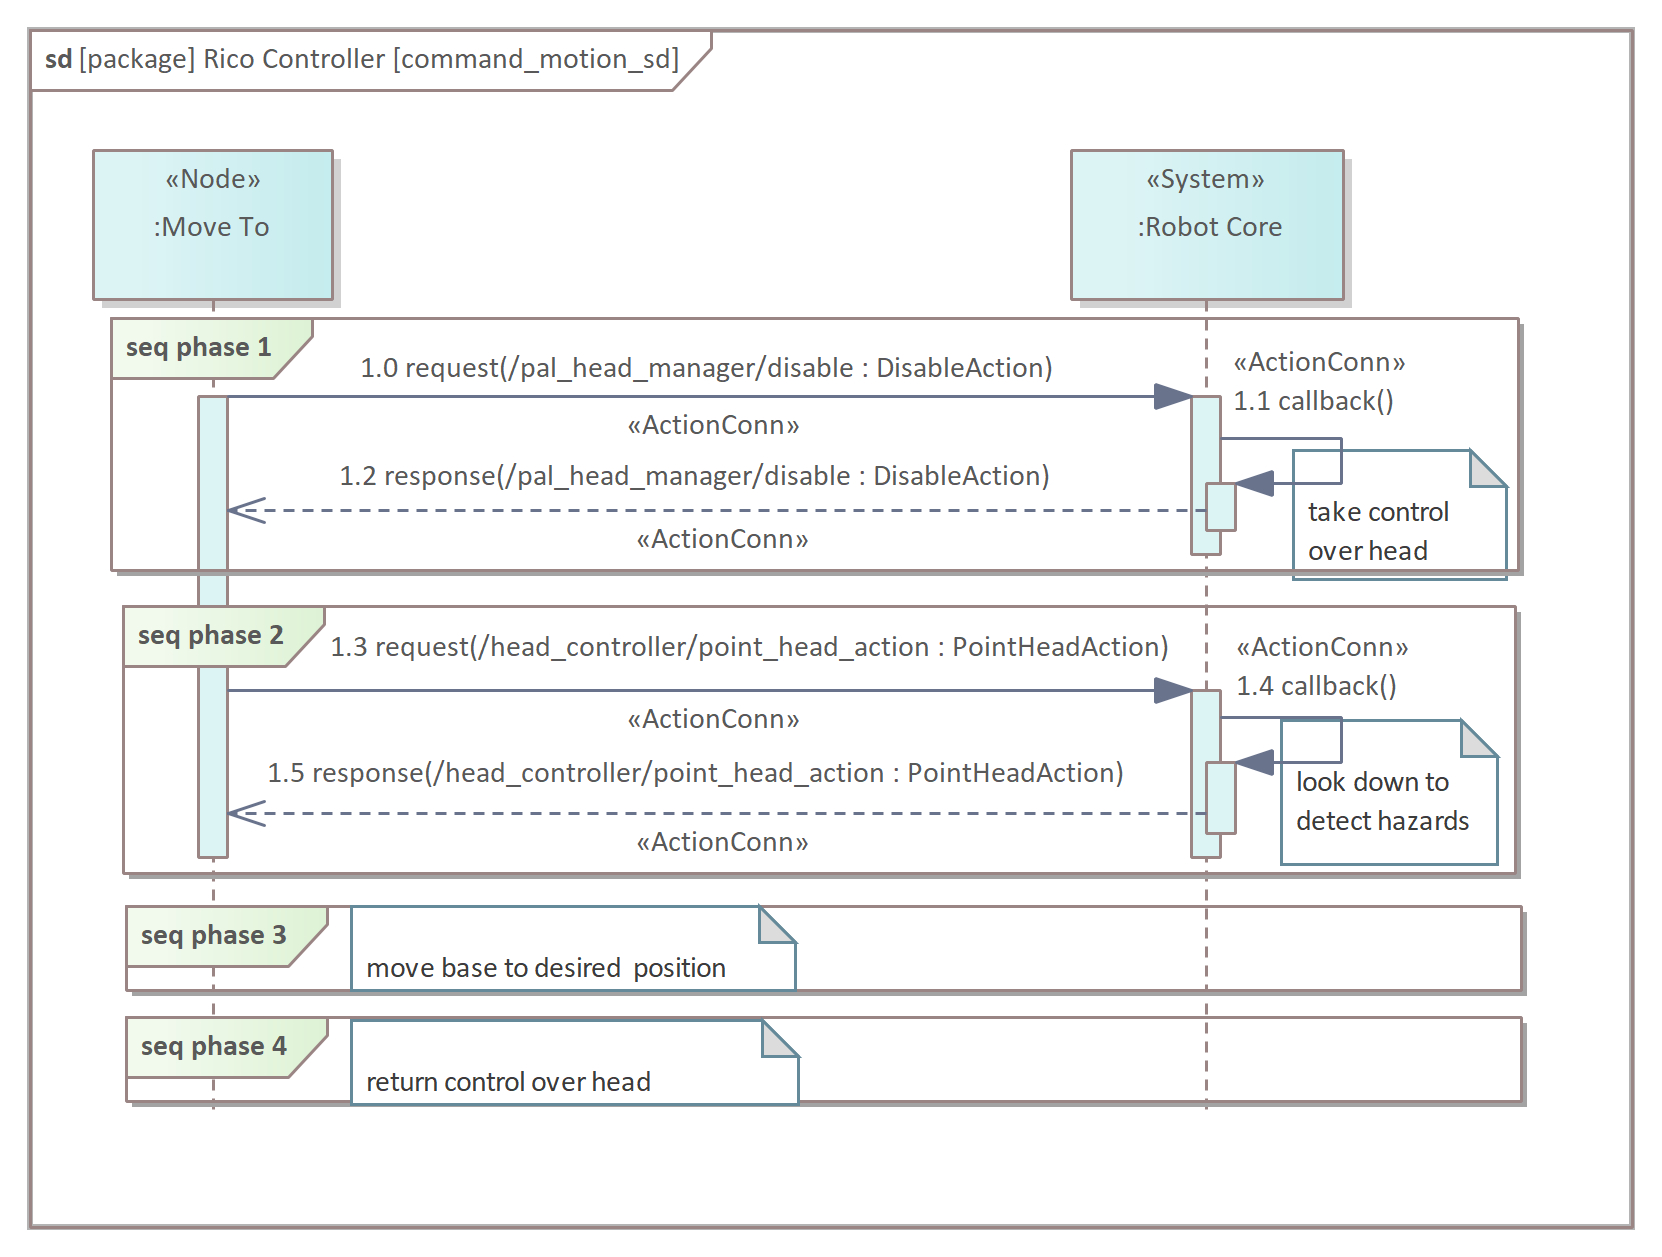
\includegraphics[scale=1.0]{img/rico_pkg/command_motion_sd.png}}
		\end{center}
		\caption{Command motion operation with detailed Communication methods presentation.} 
		\label{fig:command_motion_sd}
	\end{figure}
	
	The part of the \stWorkspace{} \texttt{:Rico} that includes previously mentioned elements is presented in Fig.~\ref{fig:rico_workspace_nodes_bdd} and Fig.~\ref{fig:rico_workspace_msgs_bdd}.
	
	\begin{figure}[H]
		\centering
		\begin{center}
			{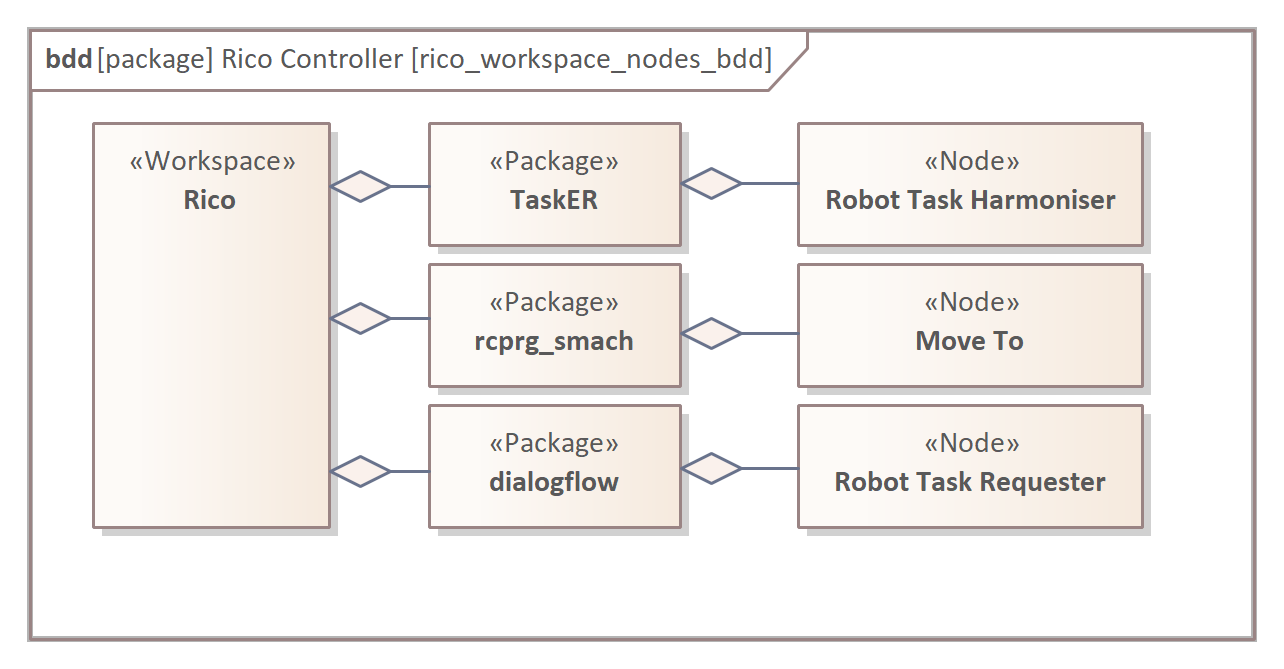
\includegraphics[scale=1.0]{img/rico_pkg/rico_workspace_nodes_bdd.png}}
		\end{center}
		\caption{Rico \stWorkspace{} composition -- Packages with Nodes.}
		\label{fig:rico_workspace_nodes_bdd}
	\end{figure}

	\begin{figure}[H]
		\centering
		\begin{center}
			{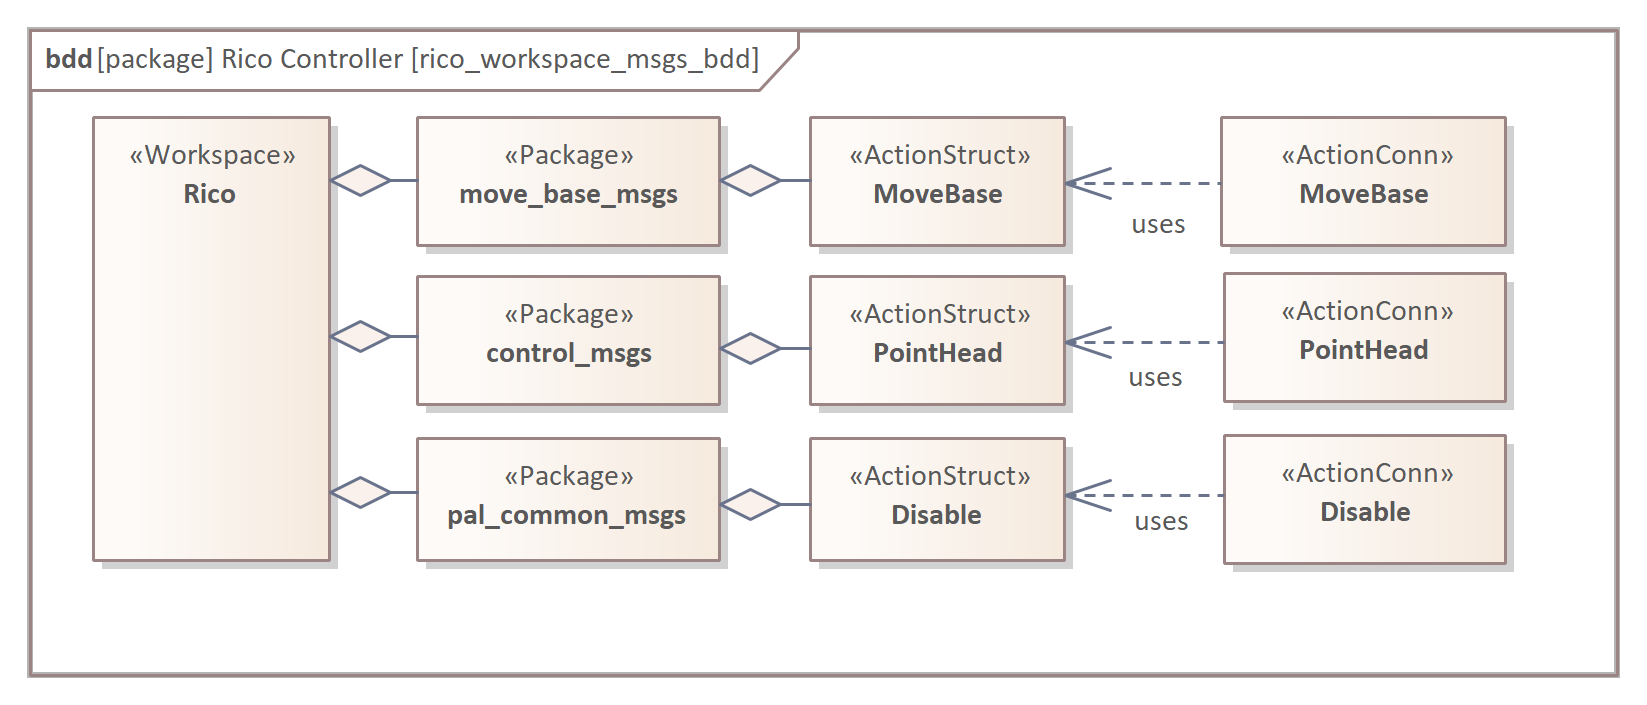
\includegraphics[scale=1.0]{img/rico_pkg/rico_workspace_msgs_bdd.png}}
		\end{center}
		\caption{Rico \stWorkspace{} composition -- Packages with Msgs.}
		\label{fig:rico_workspace_msgs_bdd}
	\end{figure}
	
			
\AtNextBibliography{\small}
\printbibliography
	
\end{document}
